\section{Идеальное дифференцирующее звено}

Рассмотрим объект управления, заданный дифференциальным уравнением:
\begin{equation}
    a_2 \ddot{y} + a_1 \dot{y} + a_0 y = u
\end{equation}

Подберем коэффициенты так, чтобы объект содержал один неустойчивый полюс: 
\begin{equation}
    \lambda_1 = 2,\quad\lambda_2 = -1 \quad\Rightarrow \quad a_2 = 1,\quad a_1 = -1, \quad a_0 = -2
\end{equation}
Кроме того, зададим начальные условия:
\begin{equation}
    y(0) = 2,\quad\dot{y}(0) = 3
\end{equation}
Рассмотрим регулятор вида: 
\begin{equation}
    u = k_0y + k_1\dot{y}
    \label{eq:conctoller1}
\end{equation}

Результат моделирования свободного движения системы представлен на рисунке \ref{fig:task1_free}.

\begin{figure}[ht!]
    \centering
    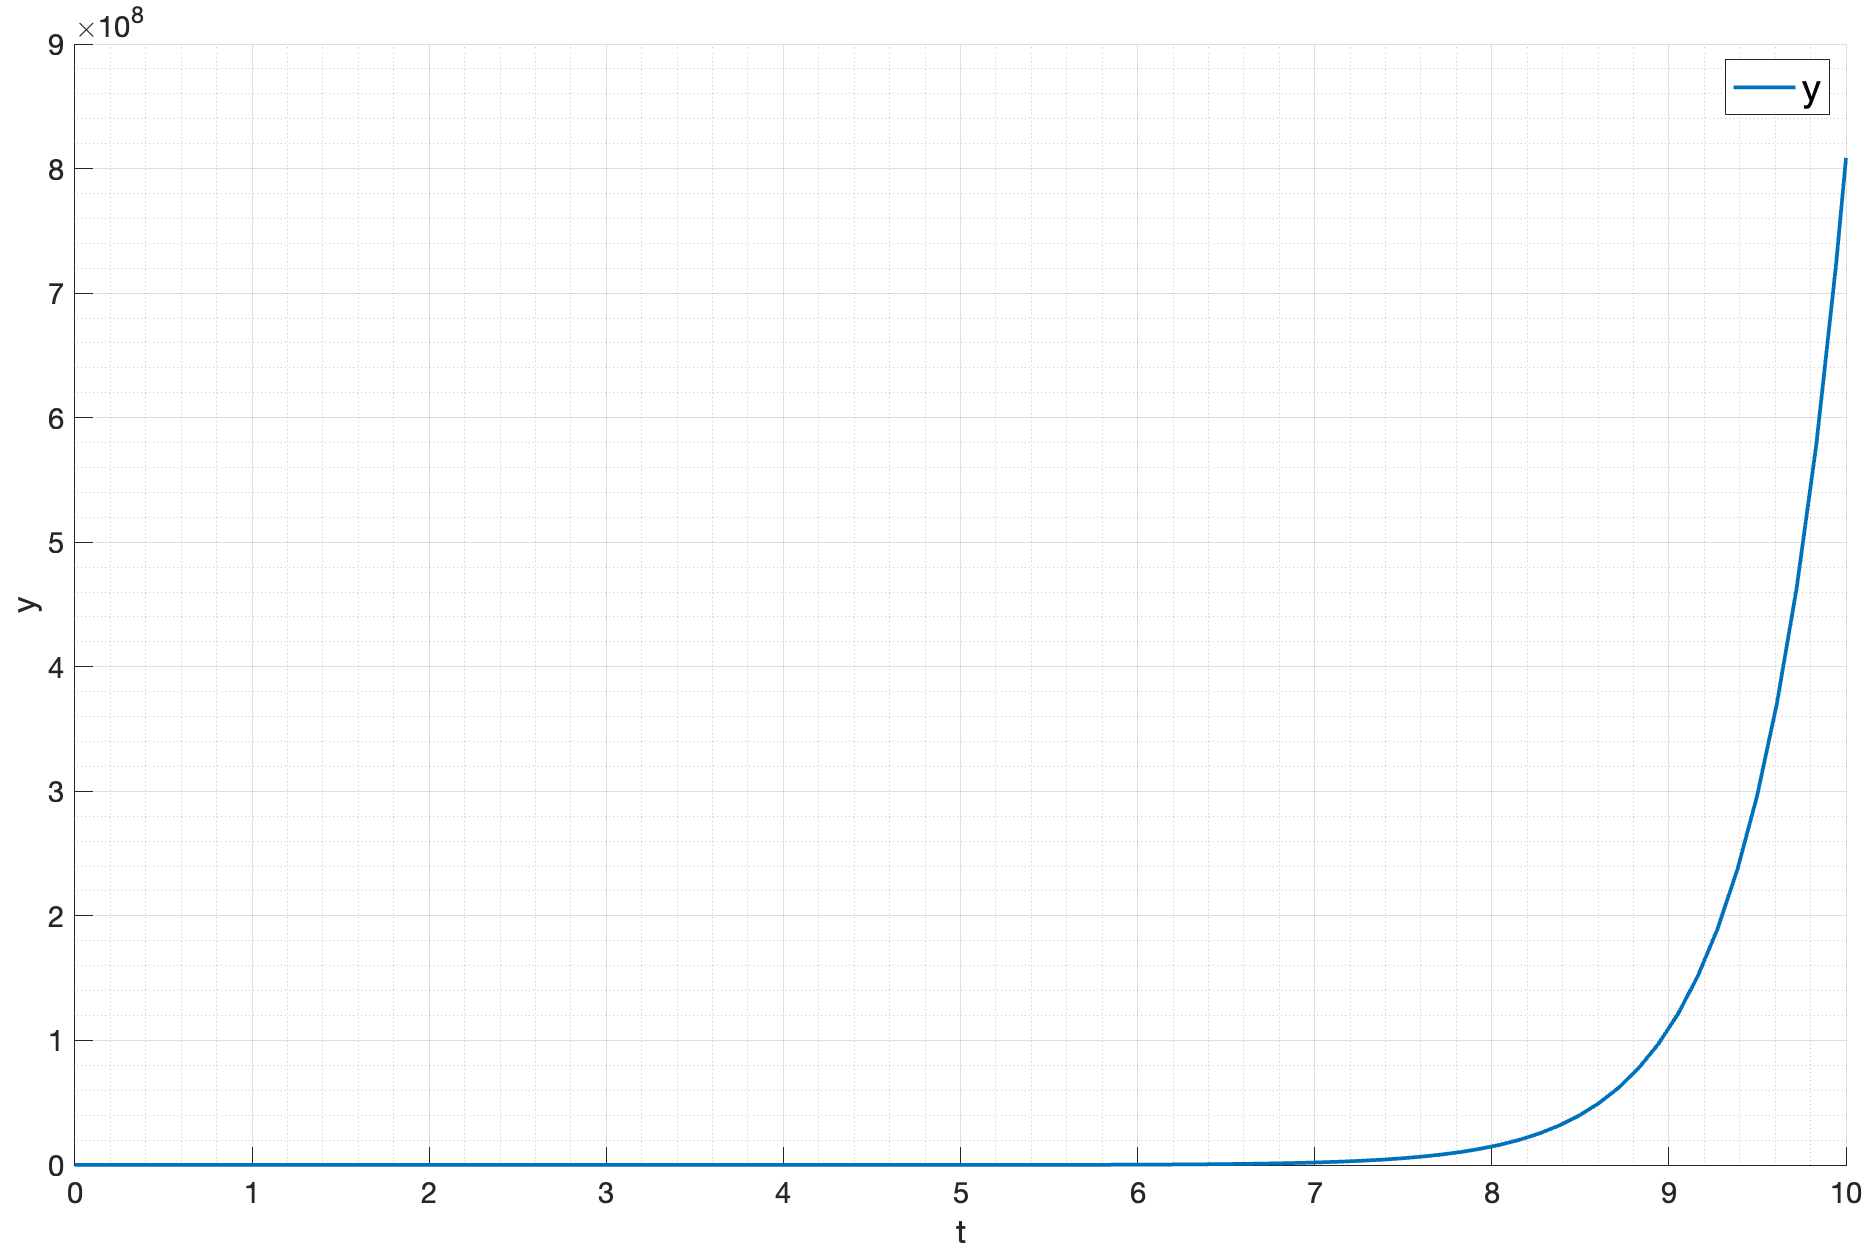
\includegraphics[width=\textwidth]{"media/plots/task1_freeout.png"}
    \caption{Свободное движение системы}
    \label{fig:task1_free}
\end{figure}

\subsection{Анализ устойчивости}
Запишем уравнение замкнутой системы:
\begin{equation}
    a_2 \ddot{y} + a_1 \dot{y} + a_0 y = k_0y + k_1\dot{y}
\end{equation}
Таким образом, можно рассматривать свободное движение системы:
\begin{equation}
    a_2 \ddot{y} + (a_1 - k_1) \dot{y} + (a_0 - k_0) y = 0
\end{equation}
Воспользуемся следствием из критерия Гурвица для системы второго порядка для 
определения границы устойчивости системы. Система будет асимптотически устойчива, если выполнено условие:
\begin{equation}
    \begin{cases}
        a_1 - k_1 > 0 \\
        a_0 - k_0 > 0
    \end{cases} \Rightarrow
    \begin{cases}
        k_1 < a_1 \\
        k_0 < a_0
    \end{cases}
\end{equation}

\subsection{Моделирование системы} 
Проведем моделирование системы при $k_0 = -3,\, k_1 = -3$.

Схема моделирования системы представлена на рисунке \ref{fig:task1_scheme}.
\begin{figure}[ht!]
    \centering
    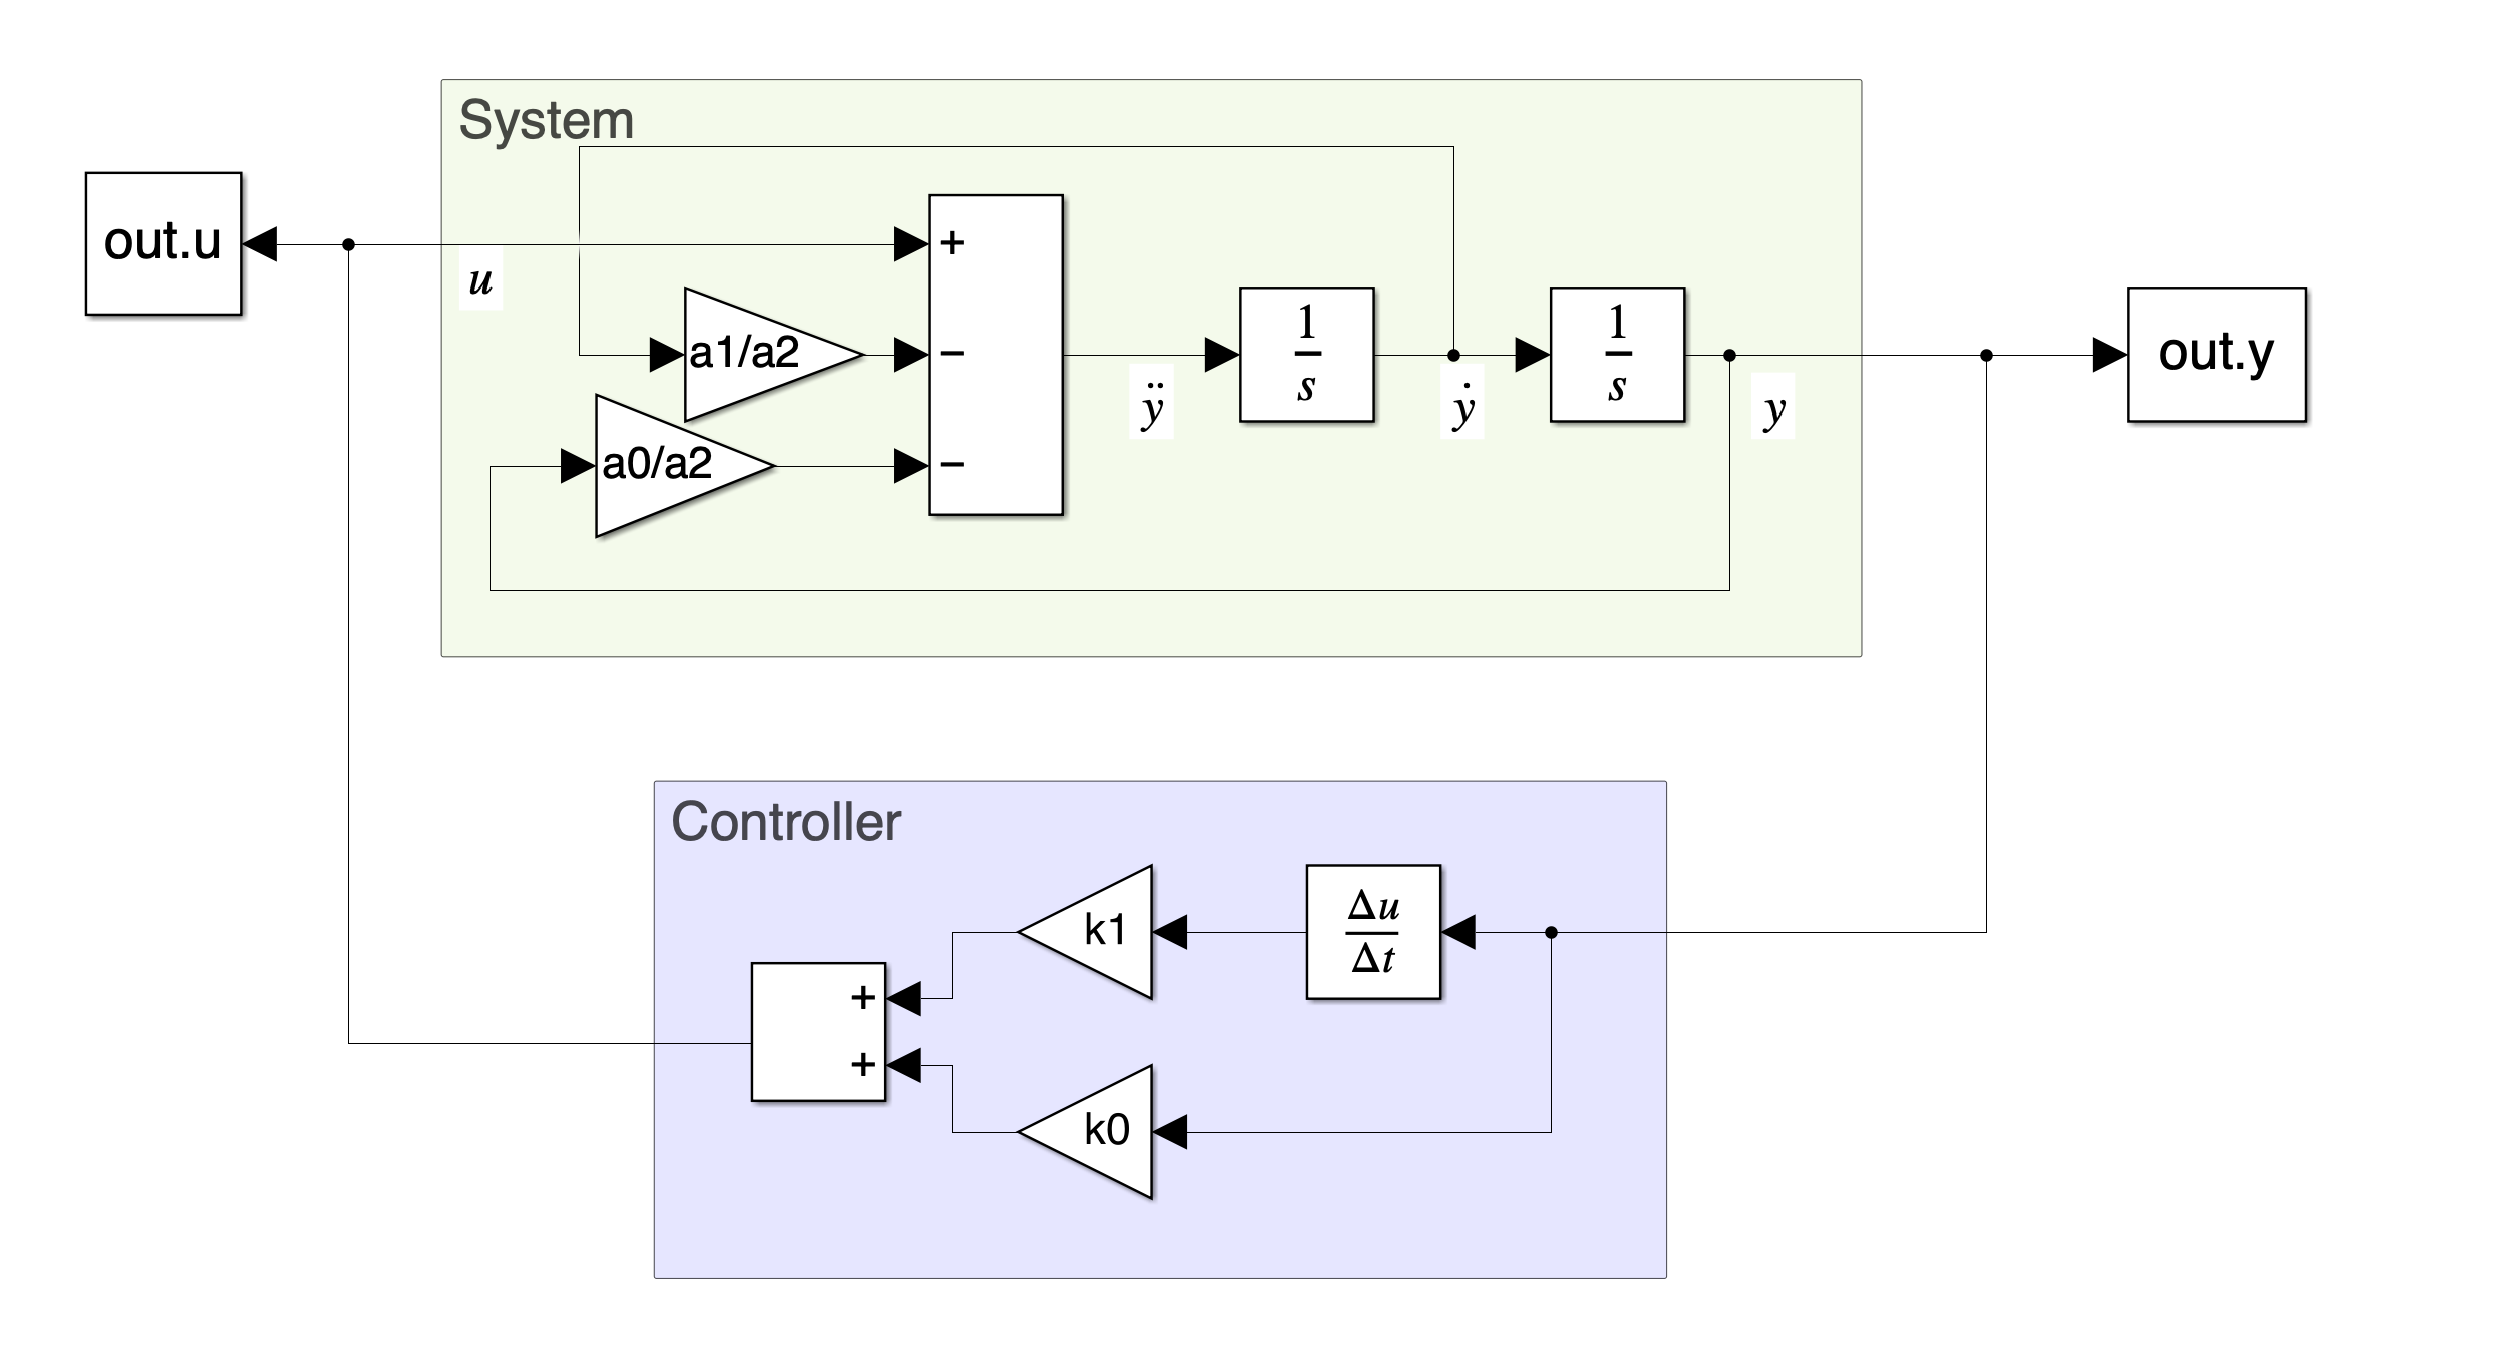
\includegraphics[width=\textwidth]{"media/scheme1.png"}
    \caption{Схема моделирования системы}
    \label{fig:task1_scheme}
\end{figure}


Результат моделирования замкнутой системы представлен на рисунке \ref{fig:task1_closed} и \ref{fig:task1_closed_in}.

\begin{figure}[ht!]
    \centering
    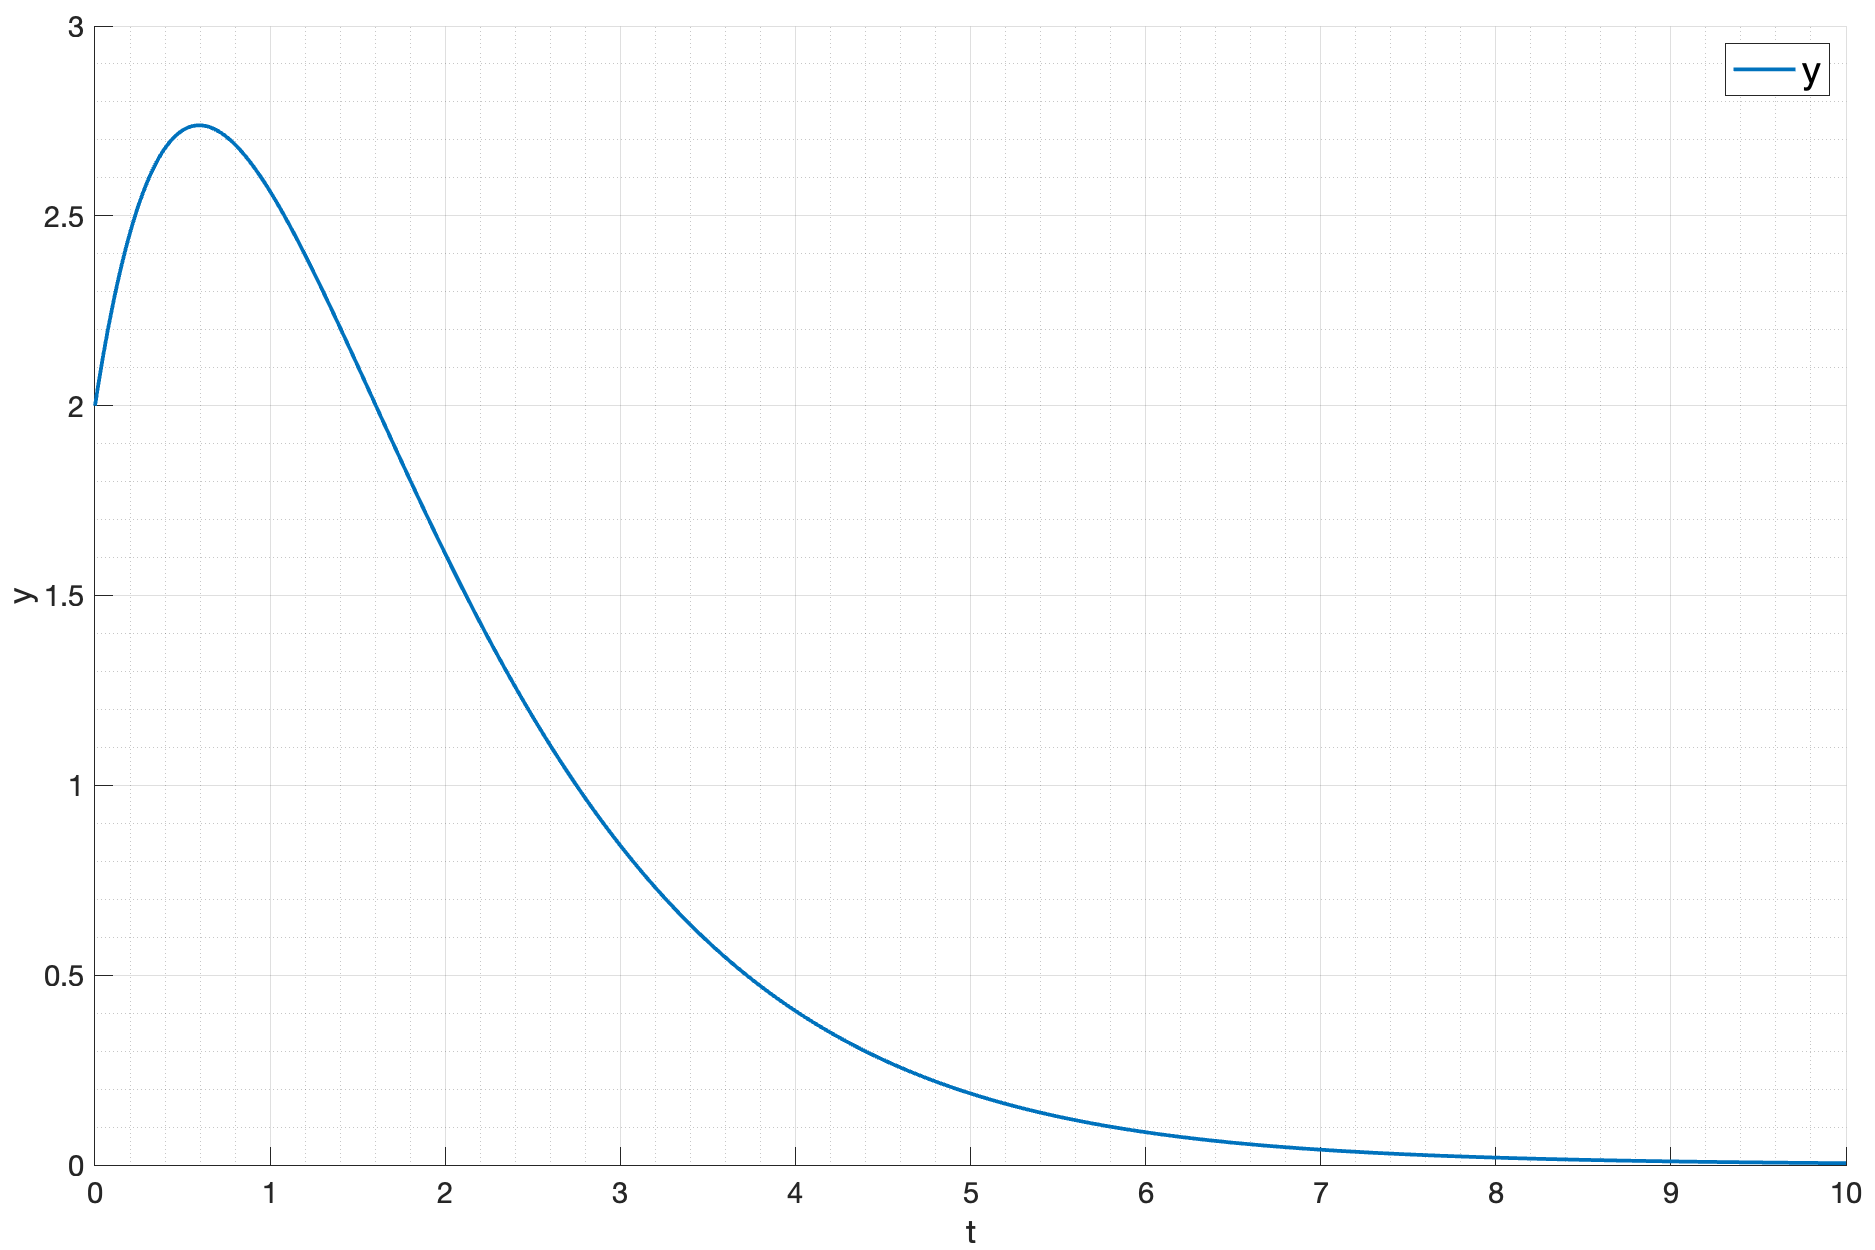
\includegraphics[width=\textwidth]{"media/plots/task1_out.png"}
    \caption{Выход замкнутой системы}
    \label{fig:task1_closed}
\end{figure}
\begin{figure}[ht!]
    \centering
    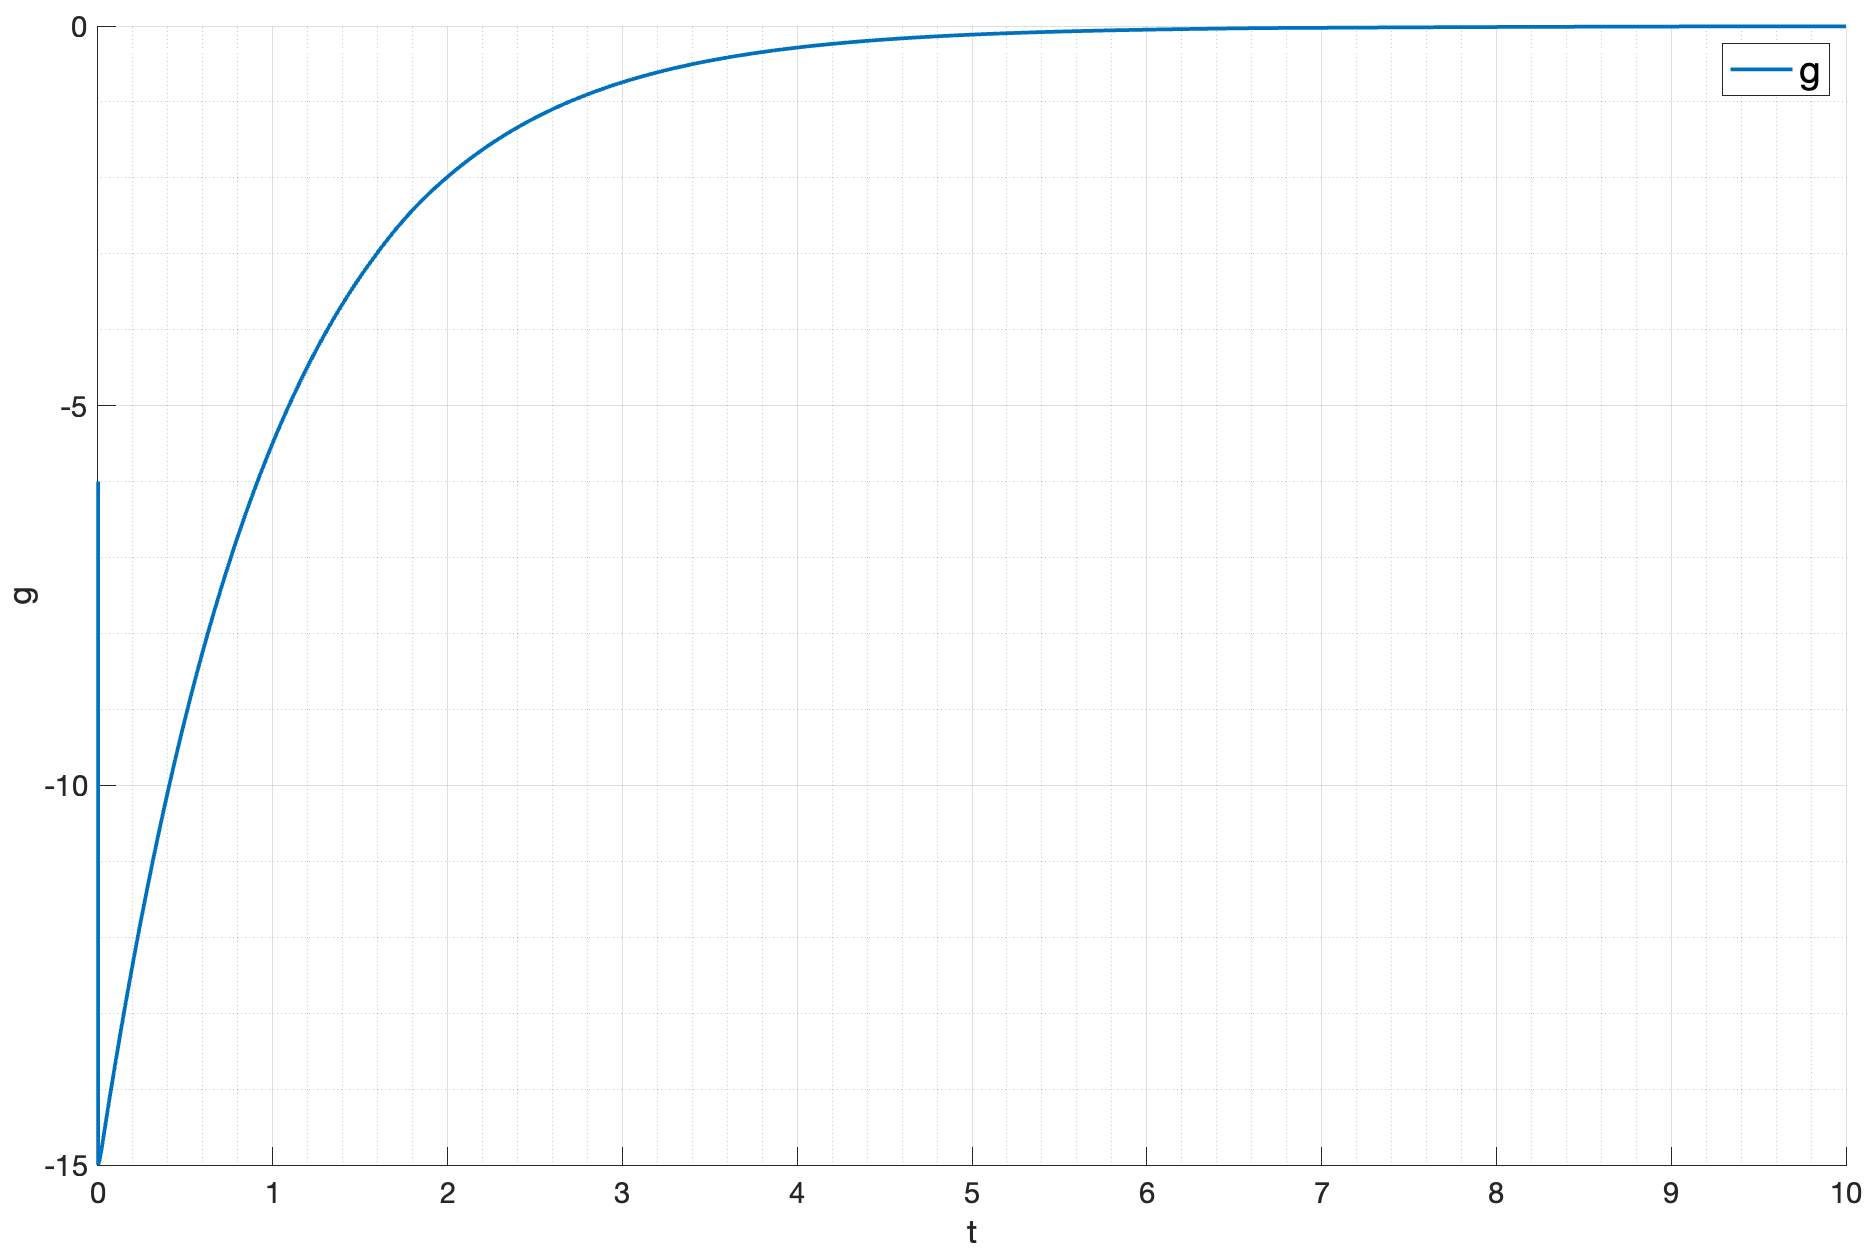
\includegraphics[width=\textwidth]{"media/plots/task1_in.png"}
    \caption{Управление замкнутой системы}
    \label{fig:task1_closed_in}
\end{figure}

Сопоставление результатов моделирования движения свободного движения и замкнутой системы показано на рисунке \ref{fig:task1_compare}.
\begin{figure}[ht!]
    \centering
    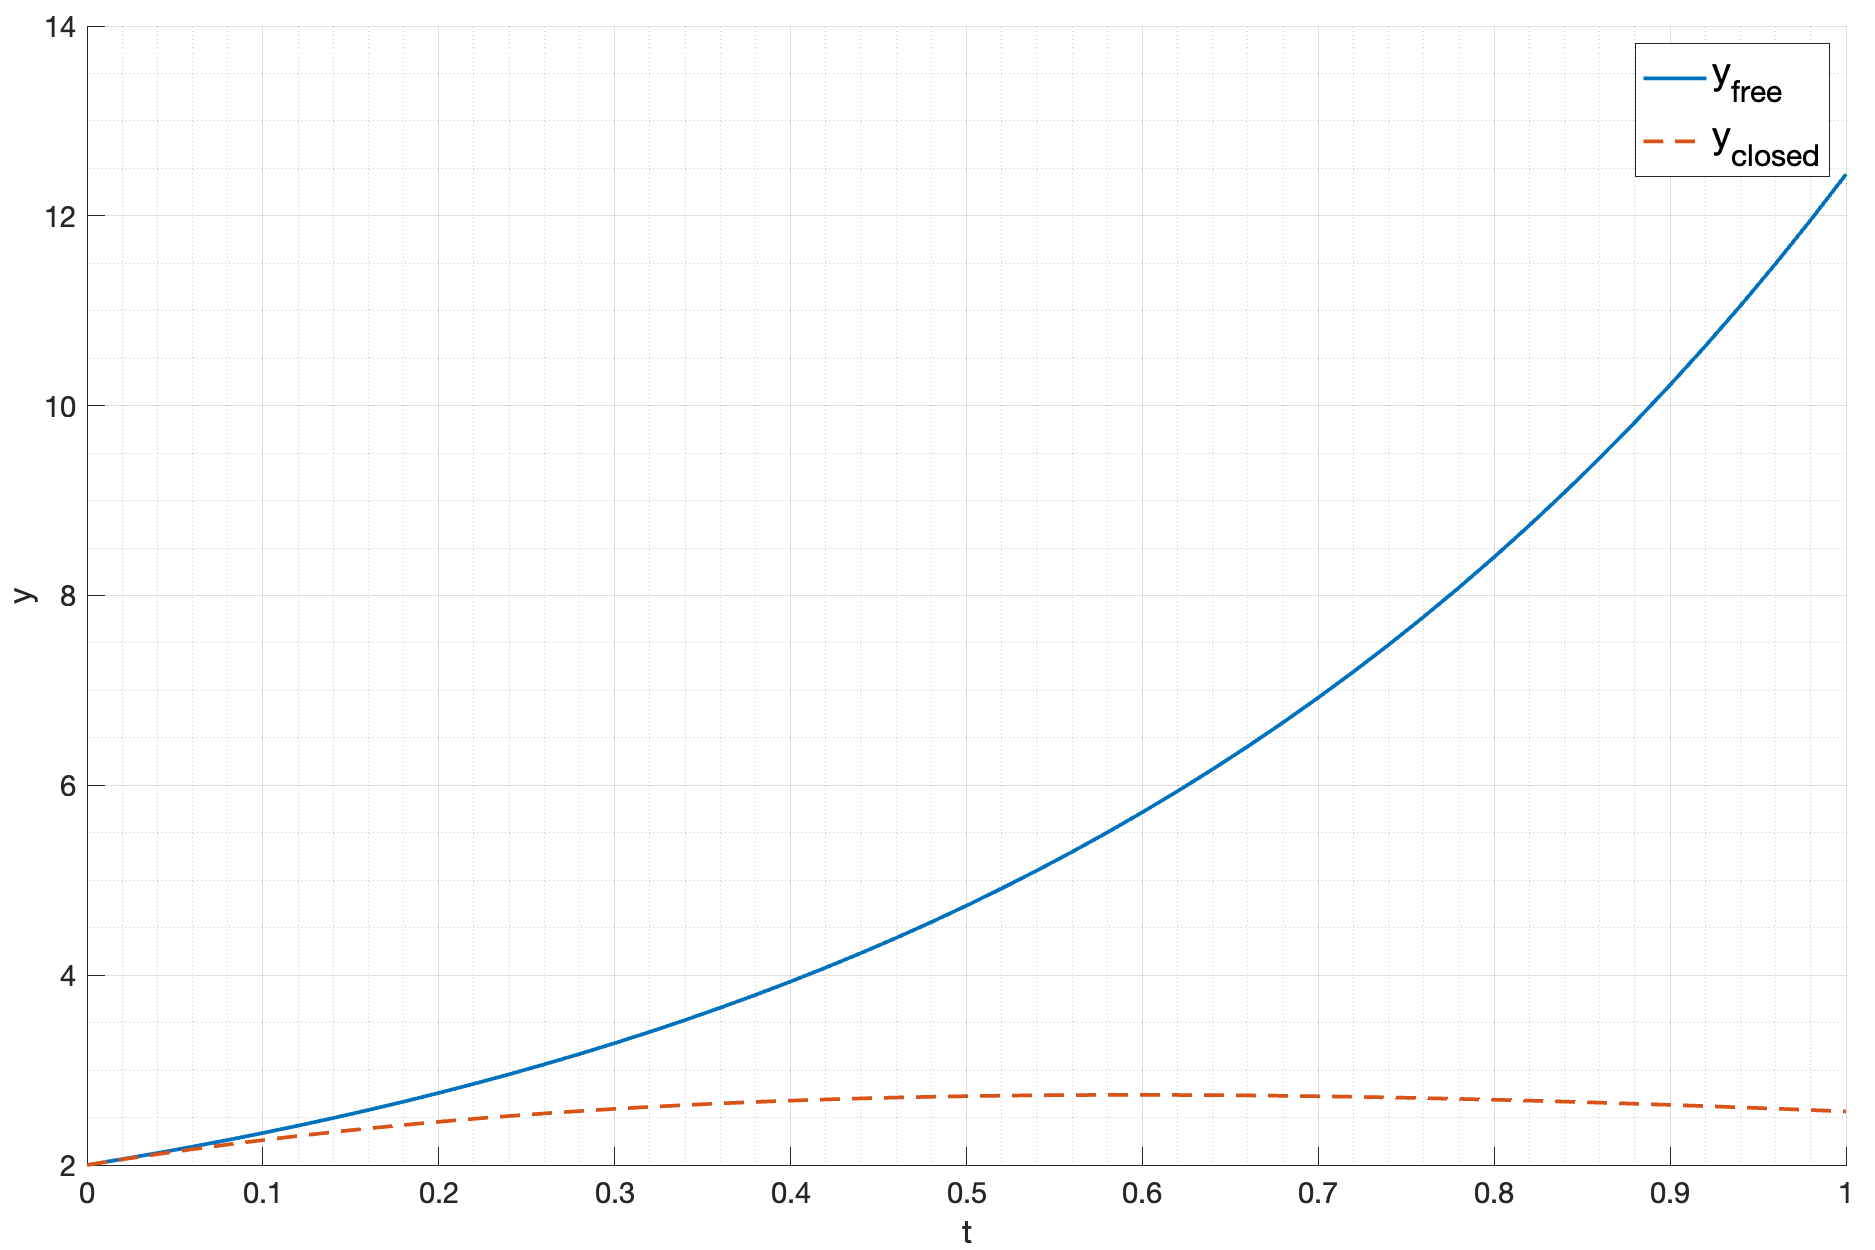
\includegraphics[width=\textwidth]{"media/plots/task1_comp.png"}
    \caption{Сравнение свободного движения и замкнутой системы}
    \label{fig:task1_compare}
\end{figure}


\subsection{Вывод}
По результатам моделирования видно, что управление смогло удержать систему в устойчивом состоянии.

